% ACL Rolling Review submission — official ACL Author Kit.
% \usepackage[review]{acl} for anonymous review (current).
% Switch to \usepackage{acl} for the camera-ready.
\documentclass[11pt]{article}
\PassOptionsToPackage{hyphens}{url}   % let long URLs break at hyphens
\usepackage[review]{acl}

\usepackage[T1]{fontenc}
\usepackage[utf8]{inputenc}
\usepackage[english]{babel}
\usepackage{times}
\usepackage{latexsym}
\usepackage{amsmath,amssymb}
\usepackage{booktabs}
\usepackage{graphicx}
\usepackage{multirow}
\usepackage{microtype}

\title{Which Pair Is It About?\\
Triple-Conditioned Verification of Literature-Mined Biotic Interactions}

\author{Anonymous ACL submission}

\begin{document}
\maketitle

\begin{abstract}
Literature-mining pipelines that populate biotic-interaction databases propose candidate
(taxon, relation, taxon) triples by co-occurrence, then decide which to keep with a
\emph{sentence-level} classifier: does this passage describe an interaction? That is the wrong
question. A candidate is retrieved precisely because its passage already names two taxa and an
interaction term, so what needs deciding is whether the passage asserts \emph{this} relation between
\emph{these two}. We test the claim with a controlled comparison: one encoder, one 48k-row
teacher-labelled corpus, three seeds, differing only in whether the model sees the candidate
triple. On 437 expert-graded candidates the triple-conditioned verifier raises per-seed AUPRC from
$0.851$ to $0.910$ and F1 from $0.775$ to $0.860$ (76 items fixed against 30 broken, McNemar
$p = 1.2\times10^{-5}$), dominating the sentence-level model at every threshold. The gain is where the argument puts it:
$+0.095$ AUPRC on passages that name three or more taxa, and none at all on passages that name
two. We decompose the residual
false positives by mechanism, show that eight deterministic candidate rules validated on training
data before evaluation raise precision from $0.825$ to $0.878$, and report the deployed two-head
configuration: F1 $0.909$ at a pre-specified threshold, at 33 candidates per second on a CPU.
\end{abstract}

\section{Introduction}
\label{sec:intro}

Biotic-interaction databases such as GloBI \citep{poelen2014global} are populated in part by text
mining. A retrieval system proposes candidate triples $(s_1, r, s_2)$ together with the passage that
allegedly supports them, and something must decide which candidates are worth a curator's attention.
The natural choice, and the common one, is a sentence-level interaction classifier: show it the
passage and ask whether it describes a biotic interaction.

That question is answered before it is asked. Candidates are proposed by co-occurrence: a passage
naming two taxa near an interaction term yields a candidate whether or not it asserts that
interaction between those two. Every candidate therefore arrives already satisfying, lexically, the
property a sentence-level classifier was trained to detect --- in the pipeline we study, on all
$175{,}588$ candidates of its retrieval pool (\S\ref{sec:setting}). What actually needs deciding is
narrower: whether the passage asserts \emph{this} relation between \emph{these two} taxa. When a
passage names three organisms, it can support one candidate and refute the other two, and a
classifier that sees only the passage must give all three the same answer.

We make this argument testable rather than rhetorical. We train the same 110M-parameter encoder on
the same teacher-labelled corpus twice, once reading the passage alone and once reading the
candidate triple as a query, and compare them on a 437-item benchmark graded by a domain expert
(\S\ref{sec:results}). Everything except the input is held fixed, so the difference between the two
is attributable to the formulation and to nothing else. The triple-conditioned model wins by a wide
and significant margin, and the gain is located exactly where the argument predicts: it is
$+0.095$ AUPRC on passages naming three or more taxa and $-0.002$ on passages naming two or fewer.

\paragraph{Contributions.}
\begin{itemize}\itemsep1pt\parskip0pt\topsep2pt
\item A controlled comparison of the sentence-level and triple-conditioned formulations on one
      encoder and one corpus, with the gain located where the argument says it should be
      (\S\ref{sec:results}).
\item A mechanism analysis of the errors that survive, including a bound showing that checking the
      triple's components separately cannot reach the largest class (\S\ref{sec:decomp}).
\item Deterministic candidate rules, each validated on 42k training rows before evaluation, that
      raise precision by $0.053$ at a recall cost of $0.020$ (\S\ref{sec:rules}).
\item A deployed two-head configuration, its threshold fixed in advance, running on a CPU
      (\S\ref{sec:deploy}), and four negative results (Appendix~\ref{sec:negative}).
\end{itemize}

\section{Setting}
\label{sec:setting}

\paragraph{Where candidates come from.}
BiotXplorer \citep{ruch2024biotxplorer} proposes candidate biotic-interaction triples from the
literature indexed by SIB Literature Services \citep{gobeill2020sibils}. For each passage it matches
taxon surface forms against a taxonomy and interaction surface forms against a vocabulary derived
from the Relation Ontology, and emits every resulting $(s_1, r, s_2)$ combination with the passage,
the matched surface strings, and their canonical forms. This is the application we build for, and
we use it only as the source of candidates: no component of it is a baseline in this paper.

\paragraph{Why the sentence-level question is constant here.}
We pulled the retrieval pool in full: $175{,}588$ candidate rows over $165{,}325$ distinct passages
and $115{,}404$ distinct triplet keys. Both taxon surface forms and the interaction surface form are
non-empty on all $175{,}588$ rows, because the presence of an interaction term is the pool's
construction filter, and an independent lexical scan for GloBI interaction vocabulary fires on
$99.82\%$ of the same passages. A classifier trained to separate passages with interaction language
from passages without it is, on this distribution, being asked about a constant. The missing input
is not an annotator artefact but the query the pipeline itself issued.

\paragraph{Benchmark.}
One benchmark of 437 rows, 246 positive, in three blocks of different provenance; we report every
block rather than pooling them into a number that hides their disagreement.
\textsc{Biotx100} is retrieved candidates, each the top-ranked candidate for its passage, graded by
a domain expert on four axes: whether each taxon surface form was correctly resolved, whether the
relation was correct, and whether the whole triple is supported by its passage. After removing three
training duplicates it contributes 97 rows, 75 positive. \textsc{Reject50} is candidates the
retrieval pipeline discarded, curated for the ones it should have kept: 41 clean rows, 9 positive.
It is the paper's recall-side instrument. \textsc{Test299} is 299 pair-level items from expert
curation, $0.542$ positive, and is where passages most often name several taxa.

The blocks do not carry the same gold. \textsc{Biotx100} is the only block graded at the level of
the whole triple; \textsc{Test299} was curated pair-level and its stored relation term was attached
by retrieval rather than by an annotator. We therefore evaluate everywhere at the level all three
share --- \emph{do these two taxa interact in this passage} --- and use the triple-level grades only to
diagnose (\S\ref{sec:decomp}). This understates what triple conditioning buys, since a candidate
with the right pair and the wrong relation counts as correct, and we prefer understating it to
scoring two blocks against a relation term nobody checked.

\paragraph{Query representation.}
Each candidate carries a canonical string and the surface form matched in the passage. On
\textsc{Biotx100} these differ for $s_1$, $s_2$ and $r$ on 34, 38 and 59 of 100 rows, and the
canonical string is absent from the passage on 31, 27 and 54. We always query with the surface form,
which is what the model can see.

\paragraph{Evaluation protocol.}
Thresholds are where this kind of evaluation goes wrong most easily, so the policy is fixed in
advance. A model's reported operating point is either \textbf{pre-specified} --- chosen on its own
training-development split, never on the benchmark --- or \textbf{block-held-out}: fitted on two of
the three source blocks and applied to the third, so that every row is scored by a threshold that
never saw it and every row is used. Comparisons between models use the same policy for both.
Intervals are $20{,}000$-sample bootstraps or Clopper--Pearson; McNemar tests carry a continuity
correction. Where three seeds exist we report the per-seed mean and standard deviation, and where we
report the average of three checkpoints' probabilities we call it an ensemble. The benchmark ships
an \texttt{in\_train} flag on 9 rows; a 5-gram Jaccard scan against all 48{,}338 training passages
finds 3 more at Jaccard $1.000$, all in \textsc{Biotx100}. All 12 are excluded throughout.

\section{Two formulations, one corpus}
\label{sec:verifier}

\paragraph{The teacher.}
Labels come from a locally hosted 32B open-weight instruction model \citep{qwen2025technical},
prompted zero-shot at temperature 0 and asked, per candidate, whether the passage supports
\emph{this} triple. Its labels therefore vary across candidates that share a passage. Against 150
human-graded items its mislabel rate is $22/150 = 14.7\%$, Clopper--Pearson $[9.4\%, 21.4\%]$, split
10 false positives and 12 false negatives.

\paragraph{The corpus.}
48{,}338 teacher-labelled rows, $0.343$ positive, drawn from the same retrieval pool as the
benchmark (disjoint passages): a 20{,}000-row base sample, 16{,}546 \emph{pair-contrast} rows,
6{,}201 actively sampled rows, and 5{,}591 rows with the candidate's argument order reversed. The
pair-contrast block is what gives the corpus its point: 2{,}017 passages enter as several rows that
are identical in the passage and differ only in the candidate and the label.

\paragraph{The two models.}
Both are BiomedBERT-base cross-encoders (110M parameters), trained for three epochs on that corpus
with the same optimiser and schedule, three seeds each, with a development split grouped on taxon
pair so that no pair spans training and development. They differ in one respect.
The \textbf{sentence-level baseline} reads the passage alone. It is the formulation a pipeline
reaches for first, and on rows that share a passage it is shown the same input with different
labels, which it cannot fit. The \textbf{triple-conditioned verifier} reads the candidate
$s_1$ \texttt{[SEP]} $r$ \texttt{[SEP]} $s_2$ as segment~A and the passage as segment~B
\citep{nogueira2019passage}, so its input moves when the candidate moves.

\section{Results}
\label{sec:results}

\begin{table}[t]\centering\small
\setlength{\tabcolsep}{3.6pt}
\begin{tabular}{lcccc}
\toprule
System & AUPRC & P & R & F1 \\
\midrule
Accept everything          & 0.563 & 0.563 & 1.000 & 0.720 \\
Sentence-level baseline    & $0.851_{\pm .006}$ & 0.730 & 0.825 & 0.775 \\
Triple-conditioned verifier & $\mathbf{0.910}_{\pm .006}$ & \textbf{0.825} & \textbf{0.898} & \textbf{0.860} \\
\bottomrule
\end{tabular}
\caption{The controlled comparison on 437 rows: one encoder, one corpus, only the input differs.
AUPRC is the per-seed mean $\pm$ standard deviation over three seeds; P/R/F1 are three-checkpoint
ensembles at block-held-out thresholds. The verifier fixes 76 items the baseline gets wrong and
breaks 30 it gets right (McNemar $p = 1.2\times10^{-5}$).}
\label{tab:main}
\end{table}

\begin{table}[t]\centering\small
\setlength{\tabcolsep}{4pt}
\begin{tabular}{lrccc}
\toprule
Passages & $n$ & Sentence & Triple & Gain \\
\midrule
naming $\le 2$ taxa & 161 & 0.876 & 0.874 & $-0.002$ \\
naming $\ge 3$ taxa & 276 & 0.846 & \textbf{0.941} & $\mathbf{+0.095}$ \\
\midrule
\textsc{Test299}  & 299 & 0.819 & \textbf{0.925} & $+0.106$ \\
\textsc{Biotx100} &  97 & \textbf{0.954} & 0.939 & $-0.015$ \\
\textsc{Reject50} &  41 & 0.465 & \textbf{0.497} & $+0.032$ \\
\bottomrule
\end{tabular}
\caption{Where the gain lives, AUPRC of the two ensembles. Taxa are counted as distinct mentions
found by a biodiversity NER model (\texttt{en\_ner\_eco\_biobert}) in the passage. \textsc{Test299}
passages name $5.1$ taxa on average, \textsc{Biotx100} $2.6$ and \textsc{Reject50} $1.7$.}
\label{tab:where}
\end{table}

\subsection{Conditioning on the triple}
\label{sec:res-main}
Table~\ref{tab:main} gives the comparison. Conditioning on the candidate triple raises per-seed
AUPRC from $0.851 \pm 0.006$ to $0.910 \pm 0.006$ and, at block-held-out thresholds, F1 from
$0.775$ to $0.860$ --- precision and recall both. On decision correctness the verifier fixes 76
items and breaks 30, McNemar $p = 1.2\times10^{-5}$. The advantage is not an artefact of where we
chose to cut: the verifier dominates the baseline at every threshold
(Figure~\ref{fig:threshold}), and at $\tau = 0.25$, for example, holds precision $0.899$ at
recall $0.793$ where the baseline holds $0.837$ at $0.687$.

Table~\ref{tab:where} locates the gain, and it is the most direct test of the paper's argument.
Split by how many distinct taxa a passage names, the two formulations are indistinguishable when it
names two or fewer --- AUPRC $0.876$ against $0.874$ --- because then there is only one pair the passage
could be about, and asking whether it describes an interaction is asking the right question. When it
names three or more, conditioning on the triple is worth $+0.095$. The blocks follow the same
pattern for the same reason: \textsc{Test299}, whose passages name $5.1$ taxa on average, gains
$0.106$, while \textsc{Biotx100}, at $2.6$ and every row the top-ranked candidate of its passage,
gains nothing.

\subsection{The query, not the encoder}
\label{sec:res-ablation}

\begin{table}[t]\centering\small
\setlength{\tabcolsep}{4pt}
\begin{tabular}{lcccc}
\toprule
Query given to the verifier & P & R & F1 & AUPRC \\
\midrule
Retrieved triple               & 0.842 & 0.890 & \textbf{0.866} & \textbf{0.912} \\
Generic relation, pair kept    & 0.876 & 0.687 & 0.770 & 0.874 \\
Relation shuffled across items & 0.879 & 0.679 & 0.766 & 0.897 \\
Relation only, no taxa         & 0.917 & 0.045 & 0.085 & 0.677 \\
Empty query                    & 0.653 & 0.191 & 0.296 & 0.641 \\
\bottomrule
\end{tabular}
\caption{Degrading segment~A of the trained verifier at inference, weights and threshold
($\tau = 0.04$) unchanged. Base rate $0.563$. Per-seed standard deviations on AUPRC are $\le 0.027$.}
\label{tab:ablation}
\end{table}

A model that reads the triple could in principle be winning on something other than the triple.
Degrading the query at inference, with weights and threshold unchanged, shows it is not
(Table~\ref{tab:ablation}). Deleting both taxa collapses ranking from $0.912$ to $0.677$ against a
base rate of $0.563$, and emptying the query entirely gives $0.641$. Replacing the retrieved
relation with a generic one, pair kept, costs $0.096$ F1; shuffling the relation across items costs
$0.100$. The decision is carried overwhelmingly by the pair and materially by the relation.

The empty-query arm is \emph{not} the sentence-level baseline: it is a model trained with the query
and deprived of it, and it does far worse ($0.641$) than a model trained without the query from the
start ($0.851$). That gap is a warning about a common shortcut. Ablating an input at inference
measures dependence on it; it does not stand in for training without it.

Neither does the gain come from the corpus's pair-contrast design. A verifier trained on the
20{,}000-row base sample alone, with the same triple-conditioned input, is indistinguishable from
the full one: per-seed AUPRC $0.9137 \pm 0.0012$ against $0.9099 \pm 0.0060$, block-held-out F1
$0.857$ against $0.860$. The input formulation is what buys the improvement; the extra supervision
buys nothing we can measure here.

\subsection{Recall side}
\label{sec:recall}
\textsc{Reject50} asks whether the candidates the retrieval pipeline discarded contain recoverable
positives. Both models recover 7 of the 9 true positives, so the sentence-level baseline is not
blind to them; what separates the two is what each lets in alongside. The baseline re-admits 15 of
the 32 correct rejections to find those 7, F1 $0.452$, and the verifier re-admits 4, F1 $0.700$.
Nine positives is a small numerator --- the Clopper--Pearson interval on $7/9$ is $[0.40, 0.97]$ ---
so we read this qualitatively: a curator mining the discarded candidates with the verifier
reviews 11 candidates of which 4 are wrong, rather than 22 of which 15 are.

\subsection{An operating curve, not a verdict}
\label{sec:opoint}

\begin{figure}[t]\centering
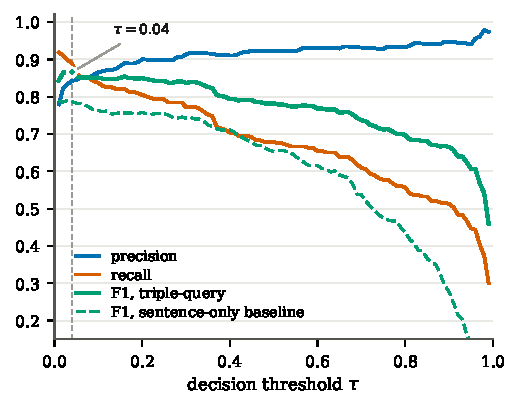
\includegraphics[width=\columnwidth]{fig/fig4_threshold.pdf}
\caption{Precision, recall and F1 of the verifier against the decision threshold on all 437 rows,
with the sentence-level baseline's F1 for comparison (same corpus and encoder). The marked threshold
is block-held-out. The verifier dominates at every $\tau$.}
\label{fig:threshold}
\end{figure}

\begin{table}[t]\centering\small
\setlength{\tabcolsep}{3.4pt}
\begin{tabular}{rcccc|ccc}
\toprule
 & \multicolumn{4}{c|}{triple-conditioned} & \multicolumn{3}{c}{sentence-level} \\
$\tau$ & keep & P & R & F1 & P & R & F1 \\
\midrule
0.01 & 290 & 0.779 & 0.919 & 0.843 & 0.690 & 0.915 & 0.787 \\
0.04 & 260 & 0.842 & 0.890 & \textbf{0.866} & 0.763 & 0.813 & \textbf{0.787} \\
0.10 & 238 & 0.866 & 0.837 & 0.851 & 0.796 & 0.732 & 0.763 \\
0.25 & 217 & 0.899 & 0.793 & 0.842 & 0.837 & 0.687 & 0.754 \\
0.50 & 181 & 0.923 & 0.679 & 0.782 & 0.866 & 0.524 & 0.653 \\
0.90 & 133 & 0.947 & 0.512 & 0.665 & 0.930 & 0.163 & 0.277 \\
\bottomrule
\end{tabular}
\caption{Both models' operating curves on all 437 rows, three-checkpoint ensembles. Rows are shown
to make the shape visible; the reported operating points are those of Table~\ref{tab:main}.}
\label{tab:curve}
\end{table}

The verifier's precision moves from $0.779$ to $0.947$ as $\tau$ moves (Table~\ref{tab:curve}), and
the right point on that curve is not a property of the model. Ingestion into a reference database
pays for false positives and belongs at the high end; assembling candidates for expert review pays
for false negatives and belongs at the low end. A filter that emits a verdict fixes that choice at
training time, for users who were never asked. A calibrated score with an adjustable threshold
leaves it to them \citep{geifman2017selective}.

\section{What the remaining errors are made of}
\label{sec:decomp}

\begin{table*}[t]\centering\small
\begin{tabular}{@{}llp{0.52\textwidth}@{}}
\toprule
Mechanism & Candidate triple & Passage (abridged) \\
\midrule
Pair-binding & (\emph{T.\ gondii}, parasite of, swine) &
``The entero-pathogenic \emph{Cystoisospora suis}, a coccidian \textbf{parasite of swine} and close
relative to \emph{Toxoplasma gondii} \ldots'' \\[1pt]
Co-listing & (katydids, prey, beetles) &
``\ldots\ remains were from insects \ldots\ (e.g.\ \textbf{beetles}, dragonflies, cockroaches, and
female \textbf{katydids}), indicating that eavesdropping on prey signals is not the only
prey-finding strategy used by this \emph{bat}.'' \\[1pt]
Negation & (wheat, hosts, \emph{F.\ acuminatum}) &
``\ldots\ \emph{F.\ acuminatum} in New Zealand was found only on \textbf{non-wheat hosts}.'' \\[1pt]
Same organism & (Chinese knotweed, pollinators, \emph{P.\ chinensis}) &
``\ldots\ potential pollinators of \textbf{Chinese knotweed (\emph{Persicaria chinensis})}.'' \\[1pt]
Entity & (\textbf{equine}, infections, human) &
``\ldots\ evidence for \textbf{equine} \emph{influenza virus} infections in human beings.'' \\
\bottomrule
\end{tabular}
\caption{One example of each mechanism among the verifier's false positives. The relation's true
argument is italicised where it is not the queried taxon; in the entity case an adjective inside a
pathogen's name was matched as the host.}
\label{tab:examples}
\end{table*}

The verifier's 47 false positives at its block-held-out operating point are not homogeneous. Read by
hand, they sort into a small number of mechanisms (Table~\ref{tab:examples}): \emph{pair-binding},
where both taxa and the relation are correct but the relation's argument is a third organism;
\emph{co-listing}, where the two taxa are members of one enumeration and interact with neither each
other nor anything in particular; \emph{negation}, where the passage asserts the opposite;
\emph{same organism}, where the two ``taxa'' are one organism named twice or an organism and its own
clade; candidates whose relation term names no biotic interaction at all (\emph{relative to},
\emph{hybridization}, \emph{migration}); and \emph{entity} failures, where a taxon string is a
taxonomic author, an organ, or an adjective inside a pathogen's name (``\emph{equine} influenza
virus''). A further handful read as gold errors and are discussed in the Limitations.

\paragraph{A bound on component-wise verification.}
The pair-binding class has a structural property worth stating, because it rules out the obvious
alternative architecture. Its members have both taxa correctly resolved \emph{and} the correct
relation; what is wrong is a binding that exists only in retrieval's combinatorics. A verifier that
checks $s_1$, $r$ and $s_2$ separately --- however good each check is --- cannot see it. On the
\textsc{Biotx100} candidates, where triple-level grades make the classes countable, 16 of the 35
unsupported candidates are pair-binding failures (the rest: 10 entity, 9 predicate). A
component-wise verifier accepting a fraction $r$ of the 65 supported triples therefore also accepts
all 16, so its precision is at most $65r/(65r+16)$: $0.802$ at full recall. Only a decision that
reads the pair \emph{in context} can go above it.

\section{Candidate rules}
\label{sec:rules}

\begin{table}[t]\centering\small
\setlength{\tabcolsep}{3.6pt}
\begin{tabular}{lccccc}
\toprule
System & P & R & F1 & fixed & broken \\
\midrule
Verifier                  & 0.825 & 0.898 & 0.860 & --- & --- \\
\quad + 7 rules           & 0.859 & 0.890 & 0.874 & 11 & 2 \\
\quad + 8 rules           & \textbf{0.878} & 0.878 & \textbf{0.878} & 17 & 5 \\
\bottomrule
\end{tabular}
\caption{Deterministic candidate rules applied before the verifier's decision, all 437 rows,
block-held-out thresholds. ``Fixed'' and ``broken'' are relative to the verifier alone; McNemar
$p = 0.027$ (7 rules) and $0.019$ (8). Both rule sets improve every block.}
\label{tab:rules}
\end{table}

Several of these mechanisms are not questions about the passage at all but about the candidate, and
a classifier is a poor instrument for them: whether two strings name one organism, whether a word is
a surname, whether ``relative to'' is an interaction. We answer those with eight deterministic
rejection rules applied to the candidate before the verifier decides. \emph{same\_organism}
(apposition of a common and a scientific name, or identical forms), \emph{own\_clade} (an adjacent
clade annotation such as ``(Acari: Prostigmata)''), and \emph{authority} (a taxonomic author parsed
as a taxon) detect the same-organism and entity classes. \emph{non\_biotic\_relation} rejects
phylogenetic, comparative and biogeographic relation terms; \emph{negated} rejects the two
negation forms whose scope provably contains one of the pair (``non-$s$ hosts'', ``no infections
with \ldots\ $s$''); \emph{not\_an\_organism} rejects organs and syndromes; \emph{pathogen\_modifier}
rejects an adjective that only ever occurs inside a pathogen's name; and \emph{co\_listed} rejects
two taxa that are conjuncts of one dependency-parsed list not governed by an interaction noun
(``interactions between $A$ and $B$'' is kept).

\paragraph{How they were validated, and what that licenses.}
No rule has a parameter fitted to evaluation labels, but rules can still be fitted by \emph{choice},
and four of these --- \emph{non\_biotic\_relation}, \emph{negated}, \emph{not\_an\_organism} and
\emph{pathogen\_modifier} --- were written after reading the false positives above. To keep their
selection from simply memorising the benchmark, every rule had to pass a criterion fixed before it
was evaluated: on the 42{,}747 training rows, at least 85\% of the candidates it rejects must be
teacher-negative, matching the teacher's own accuracy. Two first drafts failed it and were narrowed
on training data alone --- a general negation cue fired on ``without affecting the host'', and a
role-noun list rejected ``viruses'' and ``fungi'', which are legitimate coarse taxa --- and the
final rules reject teacher-negatives at $0.88$ to $1.00$ (\emph{co\_listed}, which needs a dependency
parse, on a fixed 6{,}000-row sample). The rules were then frozen, recorded by hash, and evaluated
once.

The result is in Table~\ref{tab:rules}: precision rises from $0.825$ to $0.878$ at a recall cost of
$0.020$, 17 items fixed and 5 broken, McNemar $p = 0.019$. We report it as an upper estimate, since
half the rules were chosen with these errors in view; what the training-data criterion establishes
is that they reject what they are meant to reject on 42k rows they were not chosen on, not that
their effect here would replicate exactly on new data. The three rules written before this error
analysis, from an earlier one, remove one false positive and one true positive here, which is the
honest measure of what rules carry over without being looked for.

\section{The deployed configuration}
\label{sec:deploy}

In the pipeline the verifier runs as one 110M-parameter model with two heads: the
triple-conditioned verification head described here, and a direction head that decides which taxon
is the subject, trained jointly with it and taking the pair in a canonical order so
that the direction answer cannot change when the pipeline presents the pair the other way round.
Its interaction threshold, $0.5$, is fixed on its own development split. On the 437 rows it reaches
AUPRC $0.934$ and precision $0.852$, recall $0.959$, F1 $0.902$; with the candidate rules,
precision $0.870$, recall $0.951$, F1 $0.909$.\footnote{The \emph{co\_listed} rule is omitted from
this configuration: on the joint model's accept set it removes one false positive at the cost of
three true ones.} It needs no GPU: on eight CPU threads it scores $32.7$ candidates per second with
both heads, after a one-off $7.5$\,s to load, which is faster than the pipeline retrieves them, so
every candidate is verified rather than a sample.

\section{Where the reformulation stops}
\label{sec:notfixed}

\paragraph{Entity disambiguation, and a gate that cannot fix it.}
The natural remedy for entity errors is to gate candidates on taxonomic validity. Against the Open
Tree Taxonomy \citep{rees2017opentree} such a gate catches 1 of the 35 unsupported \textsc{Biotx100}
candidates and discards 5 of the 65 supported ones. The reason is diagnostic: \emph{Illiger},
Dikarya, \emph{copia} and \emph{sulla} --- the surnames, clades, transposon families and vernacular
names behind the entity failures --- all \emph{resolve} in the taxonomy. The failure is
disambiguation, of the kind species-name normalisers address \citep{gerner2010linnaeus}, not
validity; and the gate's casualties are viruses, which are legitimate partners in this domain. The
\emph{authority} and \emph{same\_organism} rules (\S\ref{sec:rules}) target the disambiguation
directly and are the better instrument.

\paragraph{Argument order is not evaluable on this gold standard.}
Expert curation marks reversed triples as correct --- we verified two by hand,
(\emph{Breinlia}, host of, \emph{Rattus}) and (\emph{Demidospermus}, parasitized by,
\emph{A.\ inermis}) --- so no directional number on this benchmark would measure the model rather
than the convention, and the direction head's evaluation lives on corpora annotated for it. The
supervision itself is uneven in a revealing way: among the 5{,}591 reversed training rows, the rate
at which the teacher rejects a reversal is governed by the relation's \emph{surface string}.
Direction-encoding participles and prepositional forms are rejected at $0.51$--$0.70$
(\emph{affecting} $0.70$, \emph{affected by} $0.61$, \emph{parasite of} $0.57$), bare relational nouns
at $0.04$--$0.10$ (\emph{host of} $0.08$, \emph{pollinators} $0.04$). Whether supervision encodes
order at all depends on which string retrieval happened to match.

\section{Related work}
\label{sec:related}

\paragraph{Classifiers that answer an easier question.}
That a classifier can score well by exploiting how its data were assembled is among the
best-established results in NLP. Partial-input baselines recover much of the label from the
hypothesis alone in natural language inference
\citep{gururangan-etal-2018-annotation,poliak-etal-2018-hypothesis} and from the passage alone in
reading comprehension \citep{kaushik-lipton-2018-much}, and such rules hold in distribution while
failing under deployment \citep{geirhos-etal-2020-shortcut,du-etal-2024-shortcut}; the closest
task-level precedent is fact verification, where a claim-only classifier matches evidence-aware
models because of how the corpus was built \citep{schuster-etal-2019-towards}. Our sentence-level
baseline is a partial-input model in exactly this sense, and the specific feature here is that the
missing input is the query the pipeline itself issued rather than an annotator artefact
\citep{wiegand-etal-2019-detection,parmar-etal-2023-dont}. \citet{feng-etal-2019-misleading}
caution that partial-input results license claims about models and corpora rather than about
tasks, and we keep ours to the former.

\paragraph{The argument-ignoring failure is already named.}
Distant supervision assumes that a sentence containing two related entities expresses the relation
\citep{mintz2009distant}, and its standard relaxation exists because it does not
\citep{riedel2010modeling}. Since TACRED an instance has been the triple (sentence, $e_1$, $e_2$)
rather than the sentence \citep{zhang2017position}, and how the pair is injected into the encoder is
worth several F1 points \citep{soares2019matching,wu2019enriching,zhou2022improved}.
\citet{rosenman2020exposing} name our failure exactly, as an ``event heuristic'' that classifies on
(sentence, relation) while ignoring the arguments. \emph{We claim no part of that diagnosis.} What is
ours is a controlled measurement of what it costs in a verification setting built by co-occurrence
retrieval, located by block; a bound on component-wise remedies; and the candidate rules. The
entity-type shortcut usually invoked for such errors \citep{peng2020learning,mtumbuka2024entity} is
unavailable here, since both slots are filled from one inventory of taxon surface forms. Error
attribution across pipeline stages is standard and easy to get wrong
\citep{taille-etal-2020-lets,ai2023endtoend}.

\paragraph{Conditioning on the query.}
Casting a relation as a question about a named entity \citep{levy2017zero}, or as an entailment
hypothesis verbalising the relation between two of them \citep{obamuyide2018zero,sainz2021label},
is the reformulation our input format instantiates, and the resulting decision --- does this passage
support this specific claim --- has the shape of scientific claim verification
\citep{wadden2020fact}. Distilling a large model's judgments into a small student is established
practice \citep{west2022symbolic,gekhman2023trueteacher}. Selective classification thresholds a
score instead of issuing a verdict \citep{geifman2017selective}, which is how extraction is made
useful to human abstractors: \citet{swaminathan2024selective} abstain under calibrated thresholds to
automate $57$--$95\%$ of clinical chart abstraction at controlled error.

\paragraph{Text mining for interaction databases.}
GloBI \citep{poelen2014global} is populated in part by text mining \citep{dimitrova2020semantic}.
Judging an extracted fact before it reaches a curator is an old idea
\citep{rodriguezesteban2006imitating}, as is evaluating such tools by whether they help the curator
\citep{hirschman2012biocuration,britan2018nexta5,lee2018scaling}. \citet{cuzick2023interspecies},
independently, take the interacting pair rather than the passage as the annotation unit --- the unit
our pair-binding class isolates. Large language models are applied to interaction extraction at
scale \citep{keck2025extracting,farrell2024landscape,dsouza2025mining,zou2026llm}, but as
extractors: \citet{zou2026llm} standardise names and categories post hoc without checking extracted
interactions against the text that produced them. We are not aware of published work that verifies
literature-mined biotic-interaction triples against their source passage before ingestion.

\section{Conclusion}
\label{sec:conclusion}

When candidates are retrieved by co-occurrence, the sentence-level question is answered before it
is asked, and a classifier built for it is left with nothing to decide. Asking instead whether the
passage supports the candidate --- with the same encoder and the same data --- raises AUPRC from
$0.851$ to $0.910$, and the gain sits exactly where passages name more than one pair. The errors
that remain are mostly questions about the candidate rather than the passage, and deterministic
rules answer those better than a classifier does. The result is a calibrated score where a verdict
stood, cheap enough to run on every candidate.

\section*{Limitations}

\paragraph{One benchmark, singly annotated.}
437 rows in three blocks, every label assigned by one domain expert, no item graded twice: we
report no inter-annotator agreement and cannot bound label noise. Several of the verifier's most
confident false positives read as gold errors --- a bat tick ``reported \ldots\ to occasionally feed
on humans'', labelled negative. We have changed none of them: correcting gold after seeing model
output biases the evaluation toward the model, so they go instead to blind expert review, mixed
with an equal number of random controls and with model scores hidden. On the recall side the
denominator is 9 positives.

\paragraph{The rules are partly fitted by choice.}
Four of the eight rules were selected after reading this benchmark's false positives
(\S\ref{sec:rules}). The training-data criterion bounds how much that selection can have memorised
the benchmark, but it does not remove it, and the rules' $p = 0.019$ should be read as optimistic
until it is confirmed on candidates neither the rules nor their author have seen. The rules also fire
on no row of a separate 100-candidate development sample, so that sample can neither confirm nor
contradict them.

\paragraph{Fresh candidates are harder.}
On that development sample --- 100 retrieved candidates drawn after the benchmark, half of them
from passages containing several candidate pairs --- the verifier reaches F1 $0.698$, well below its
benchmark figure. Its label provenance is not identical to the benchmark's, so we do not read this as a
measured drop, but it is the clearest sign that multi-pair passages remain the hard case and that the
benchmark may understate their share of a live pool.

\paragraph{The diagnosis is triple-level; the evaluation is pair-level.}
Only \textsc{Biotx100} carries whole-triple gold. Evaluating at the pair level everywhere means a
candidate with the right pair and a misbound relation counts as correct, so the headline understates
what triple conditioning buys; triple-level gold on the other two blocks would sharpen it.

\paragraph{Teacher noise and pretraining exposure.}
The training labels come from a prompted teacher wrong about one time in seven, and the student
inherits that boundary; training on model-generated labels can degrade encoders
\citep{lu2025feeding}. The passages are published MEDLINE text and the teacher is a pretrained
model, so we cannot exclude that it saw them, and its labels may be optimistic for genuinely new
literature.

\paragraph{Upstream failures are out of reach.}
Of the 50 candidates the retrieval pipeline discarded, 32 carry an incorrect interaction term and 17
a mis-resolved taxon, 14 of them both. Those fail before any verifier is consulted, and no change to
the decision stage, ours included, addresses them.

\paragraph{One system, one domain.}
One retrieval system, one interaction vocabulary, taxon--taxon interactions in MEDLINE. The mechanism
--- a pair-agnostic decision over passages that name several candidate pairs --- is not specific to
ours, but we have not shown that other pools fail the same way.

\bibliographystyle{acl_natbib}
\bibliography{references}

\appendix

\section{Per-seed results}
\label{app:seeds}

\begin{table}[h]\centering\small
\begin{tabular}{lcc|cc}
\toprule
 & \multicolumn{2}{c|}{triple-conditioned} & \multicolumn{2}{c}{sentence-level} \\
 & AUPRC & F1 @ 0.5 & AUPRC & F1 @ 0.5 \\
\midrule
seed 1 & 0.9140 & 0.7832 & 0.8578 & 0.6321 \\
seed 2 & 0.9030 & 0.8018 & 0.8513 & 0.6976 \\
seed 3 & 0.9128 & 0.7755 & 0.8449 & 0.6633 \\
\midrule
mean $\pm$ sd & $0.9099 \pm 0.0060$ & $0.7868 \pm 0.0136$ & $0.8513 \pm 0.0064$ & $0.6643 \pm 0.0328$ \\
ensemble & 0.9123 & 0.7822 & --- & --- \\
\bottomrule
\end{tabular}
\caption{Per-seed figures. The ensemble averages three checkpoints' probabilities and is what the
body of the paper reports at operating points.}
\label{tab:perseed}
\end{table}

\section{Negative results and cost}
\label{sec:negative}

\begin{table}[h]\centering\small
\setlength{\tabcolsep}{3pt}
\begin{tabular}{@{}lp{0.27\columnwidth}p{0.30\columnwidth}@{}}
\toprule
Intervention & Benefit & Cost \\
\midrule
Taxon-validity gate & 1 of 35 unsupported caught & $-5/65$ supported; rejects viruses \\
Self-distillation & none & $-0.001$ P, $-0.008$ F1 \\
6-layer compression & $1.9\times$ CPU throughput & $-0.088$ precision \\
Corpus signal-matching & none & $-0.059$ AUPRC \\
Rule-family training data & none & AUPRC $+0.005$ to $-0.037$ \\
\bottomrule
\end{tabular}
\caption{Five plausible design choices that measurably do not pay.}
\label{tab:negative}
\end{table}

Table~\ref{tab:negative} collects interventions that did not pay, because each is a plausible first
thing to try. Self-distillation at equal capacity is null, suggesting the teacher's knowledge is
already saturated in the student. Compression to six layers buys throughput the pipeline does not
need for $0.088$ precision. Reweighting the corpus toward the deployment signal distribution cost
$0.059$ AUPRC. Most instructive is the last row: before the candidate rules existed, we turned the
same mechanisms into \emph{training data} --- synthetic negatives for the same-organism, own-clade and
authority classes, and in a second variant for co-listing --- and retrained. The first variant left
AUPRC unchanged within seed noise and the second cost $0.037$. Mechanisms that are properties of the
candidate are better answered by a rule than taught to a classifier. Deltas in the first four rows
were measured under an earlier version of the evaluation and are given as directions.

\end{document}
